\chapter{NOOSFERO}

O Noosfero é uma plataforma \textit{open source} para a construção de redes sociais
e colaborativas. Desenvolvido em Ruby on Rails e licenciado sob AGPL versão 3, o
projeto ainda conta com desenvolvimento ativo.

Além dos mecanismos de interação social, o Noosfero também conta com um sistema de
gerenciamento de conteúdo, o que possibilita a criação de \textit{blogs} e o
compartilhamento de arquivos. A plataforma também pode ser estendida por
\textit{plugins} desenvolvidos pela comunidade, e conta com o conceito de ambientes,
que permitem a criação de diversas redes isoladas funcionando sobre uma mesma
instância da aplicação.

\begin{figure}[h]
	\centering
		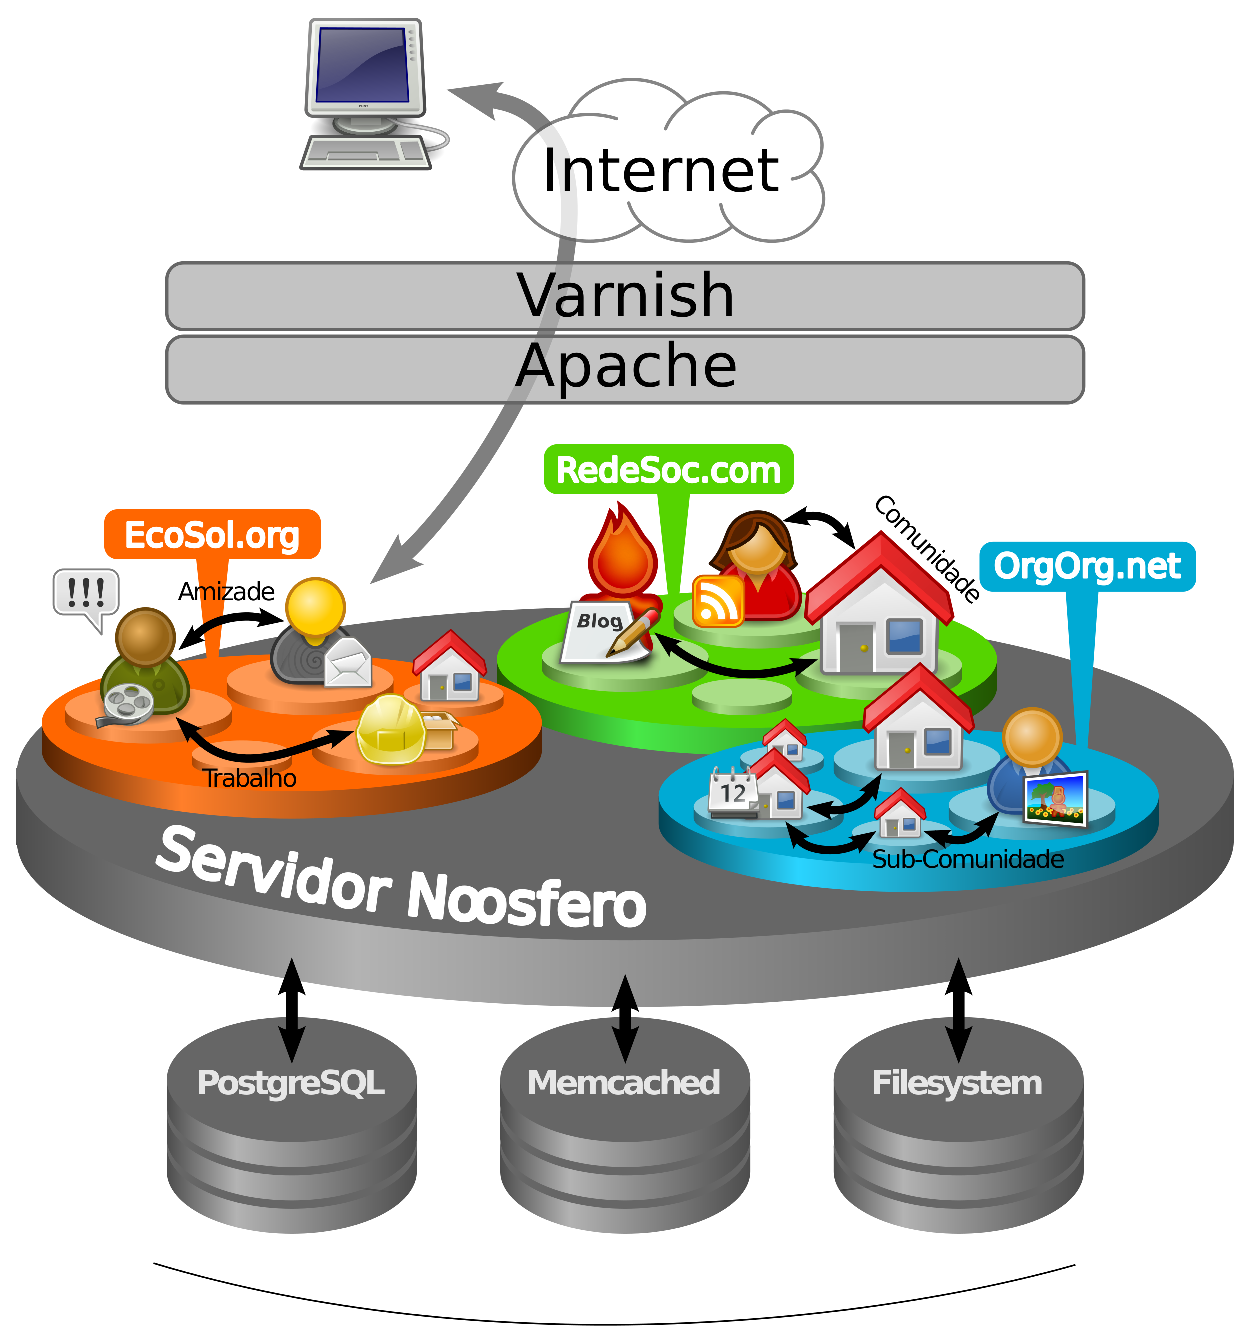
\includegraphics[keepaspectratio=true,scale=0.4]{figuras/noosfero_estrutura.eps}
	\caption{Arquitetura do Noosfero}
	\label{fig:noosferoEstrutura}
\end{figure}
% adicionar fonte

As informações e publicações de pessoas e organizações podem ser públicas ou
privadas. Já os relacionamentos entre estas entidades podem ser tanto simétricos
como assimétricos.

Enquanto um relacionamento simétrico depende da concordância de ambas as partes para
o compartilhamento das informações privadas (como por exemplo amizades ou
filiações), um relacionamento assimétrico depende apenas do interesse de uma das
entidades em acompanhar as informações públicas de algum perfil (como no caso da
funcionalidade de seguidores).



\section{SUPORTE À FEDERAÇÃO}

As definições da federação no Noosfero surgiram no contexto de desenvolvimento do
projeto do Portal do Software Público, como resultado de uma consultoria executada
pela Cooperativa de Tecnologias Livres \cite{colivre2016}. O produto foi um
relatório que define os objetivos e requisitos da implementação de federação na
plataforma Noosfero.

A proposta é que seja possível realizar a integração não só com outras instâncias do
Noosfero, como também com outras redes sociais. Desta forma, é necessário adotar
especificações que tenham o mínimo de aderência na comunidade, ao menos em outros
projetos que investem na implementação da federação entre redes sociais. Os
protocolos Diaspora e OStatus foram escolhidos observando projetos como o Hubzilla,
Friendica, e o próprio Diaspora.

É interessante que mesmo a integração entre redes Noosfero respeite os padrões
adotados pelos protocolos de referência, evitando a criação de outro padrão que não
reconhecido pelo restante dos projetos. No entanto, implementar a federação
respeitando os padrões existentes pode exigir uma refatoração da arquitetura ou das
funcionalidades da plataforma. Por exemplo, nenhum dos protocolos de referência
respeita o conceito de relacionamentos simétricos, padrão no Noosfero até então.


\subsection{Federação entre redes Noosfero}

As primeiras contribuições com a federação no Noosfero foram na integração de
instâncias diferentes da plataforma. As atividades foram definidas de acordo com
um \textit{roadmap} que dividiu a implementação em quatro fases, que cobrem desde
a reestruturação da arquitetura da aplicação, até a construção dos mecanismos
necessários para a autenticação e relação entre as redes.

% TODO: que funcionalidades devem ser oferecidas para um usuário federado

O protocolo construído entre redes Noosfero é baseado nas especificações do
WebFinger e OAuth para a descoberta de identidade e autorização de perfis,
respectivamente. Em relação à comunicação entre as redes, o protocolo Diaspora foi
definido como referência. 

\subsubsection{Fase 1: preparação}

Até a versão 1.5 do Noosfero, todos os relacionamentos entre as entidades da rede
eram baseados no conceito de relacionamento simétrico. No entanto, as demais redes
federadas, e a maioria dos padrões mais implementados, trabalham apenas com o
conceito de relacionamentos assimétricos, o que incentivou o desenvolvimento da
funcionalidade de seguidores no Noosfero.

Na fase de preparação foram introduzidos os relacionamentos assimétricos através
desta funcionalidade. Os seguidores são notificados a respeito de atividades
públicas de perfis seguidos. No Noosfero, cada perfil pode permitir ou não que
usuários o sigam. Usuários por sua vez organizam seus seguidores em círculos,
categorizando suas relações.

\subsubsection{Fase 2: intercomunicações}

% TODO: detalhar o conceito do ExternalPerson?

Durante a fase de intercomunicações foi construída a infraestrutura básica para a
integração entre redes Noosfero. O conceito de ambientes e usuários externos foram
introduzidos à arquitetura do Noosfero, que passa a considerar a ação de usuários
que não possuem perfis locais sobre a aplicação.

Nesta fase também foi implementada a especificação do WebFinger, que já está sendo
utilizada para a descoberta de usuários na autenticação entre redes Noosfero.

% TODO: adicionar nota de rodapé do directory.noosfero.org
Inicialmente, apenas as redes listadas no diretório central do Noosfero podem ser
habilitadas no painel de administração da federação. A descentralização desta lista
ou a automatização do processo de descoberta não fizeram parte do planejamento
inicial.

\subsubsection{Fase 3: integração externa}

A fase de integração externa teve como objetivo aproveitar a infraestrutura de
usuários externos para autenticar usuários de outros serviços sem a necessidade de
perfis locais. Com isto, usuários de sistemas que suportem OAuth podem acessar o
Noosfero, consumir conteúdo, e executar um conjunto limitado de ações.

Durante esta etapa, o \textit{plugin} que torna o Noosfero em um cliente OAuth foi
evoluído para permitir que usuários possam tanto criar um perfil local a partir das
informações da rede de origem, como também apenas acessar o Noosfero com um perfil
temporário. Por enquanto, os únicos fornecedores OAuth suportados são o Google,
Facebook, Twitter, GitHub, e o próprio Noosfero. No entanto, novos fornecedores
podem ser facilmente adicionados.

\subsubsection{Fase 4: inter-relações}

% Relações entre usuários de diferentes redes
A última fase de desenvolvimento da federação de redes Noosfero foi permitir o
relacionamento entre usuários de instâncias diferentes. De modo geral, esta fase
consistiu em permitir que usuários externos sejam capazes de seguir perfis, comentar
conteúdos, e publicar em murais de outros usuários.

% TODO: detalhar mais do ponto de vista da implementação

De forma a permitir relações entre usuários federados foi necessário refatorar a
funcionalidade de seguidores, adicionando o suporte a perfis externos. Outro ponto
fundamental é a capacidade de mandar mensagens entre instâncias do Noosfero,
possibilitando o envio de notificações necessárias em todas as interações entre
usuários externos e perfis.

% TODO: explicar o mecanismo de troca de mensagens

Com a conclusão desta fase, um usuário de qualquer rede Noosfero pode se autenticar
em uma instância diferente da original, e executar interações básicas com outros
perfis, como por exemplo comentar uma publicação ou seguir a atividade de uma
comunidade. As interações exercem impacto sobre as redes de todos os usuários
envolvidos, e todos os conteúdos compartilhados devem apresentar o mesmo estado.


\subsection{Federação com outras redes sociais}

A implementação da federação com redes não Noosfero devem usar a infraestrutura
desenvolvida para a integração entre redes Noosfero, principalmente os mecanismos
de usuários externos e troca de mensagens.

% TODO: essas aplicações foram escolhidas com base em que?
Já que não existe um padrão para a federação de redes sociais, inicialmente é
necessário oferecer suporte a aplicações individuais. Dedicou-se atenção especial
aos projetos que contam com iniciativas de federação significativas, precisamente
os projetos Diaspora, Hubzilla, Friendica, e GNU Social.

% TODO: adicionar referência para o suporte que os projetos oferecem (nota de rodapé)
Com exceção do GNU Social, os projetos que serão inicialmente suportados atendem às
especificações do protocolo Diaspora. O suporte às redes baseadas no OStatus será
oferecido implementando uma parte dos protocolos desta suíte, como o Salmon, o
Activity Streams e o PubHubSub.

Para que a federação seja bem sucedida, é essencial garantir que a integração seja
bidirecional. Além de permitir que usuários acessem e interajam com uma rede
Noosfero com o perfil de outra rede social, um usuário Noosfero também devem
conseguir fazer o mesmo em qualquer uma destas redes. Além da autorização, a
federação depende da descentralização dos conteúdos, o que exige que as interações
possam acontecer em qualquer uma das redes, mas que o estado seja sempre o mesmo
em cada uma delas.

De modo geral, as mesmas funcionalidades implementadas na federação de redes
Noosfero deve ser suportada, desde que toda interação exerça impacto tanto na rede
de origem quanto na rede federada, sejam estas instâncias Noosfero ou não.

As atividades necessárias para a implementação desta etapa de federação podem ser
organizadas com base nos marcos a seguir.

% TODO: revisar marcos
% TODO: o que o Diaspora suporta e não suporta?
% TODO: o que especificamente deve ser implementado no OStatus?

\begin{enumerate}
  \item{Possibilitar o gerenciamento das redes federadas através de um  mecanismo de 
        \textit{whitelist} para a autorização de redes não Noosfero, o que deve
        incluir a avaliação de um mecanismo de descoberta para as redes existentes;}

  \item{Possibilitar um usuário possa acessar outras redes com as credenciais de sua
        rede de origem, sem a necessidade de um novo cadastro;}
        % Evolução do plugin de OAuth ou utilização do WebFinger?

  \item{Permitir relações assimétricas entre usuários de redes distintas através do
        protocolo Diaspora. Permitir que as atividades (\textit{feed}) sejam
        visualizadas tanto na redes de origem quanto na federada;}

  \item{Possibilitar interações a partir de qualquer uma das redes através do
        protocolo Diaspora, o que evita que, por exemplo, um usuário precise acessar
        outro domínio para comentar uma publicação. Os usuários envolvidos na
        interação devem ser notificados em suas redes de origem.}

  \item{Permitir relações assimétricas e interações através dos protocolos indicados
        na especificação do OStatus, com os mesmos fins da implementação através do
        Diaspora;}
\end{enumerate}

% TODO: (no caso do Diaspora: o que inclui tais e tais funcionalidades...)
No desenvolvimento deste trabalho será priorizada a implementação da federação
através do protocolo Diaspora. Indica-se a expansão da federação por meio do OStatus
como um trabalho futuro.

\subsubsection{Implementação do Protocolo Diaspora}

% o que o Noosfero precisa ter

O protocolo Diaspora está implementado no formato de uma \textit{gem}, que pode ser
facilmente adicionado como uma dependência em projetos que utilizem a plataforma
\textit{Ruby on Rails}, como o Noosfero. A \textit{gem} é mantida pela mesma
comunidade que mantém o projeto original, e sempre acompanha a última especificação
adotada.

% adicionar nota relatando problemas com o avanço da Gem, quebrando plataformas
% que a utilizem

% TODO: adicionar nota de rodapé explicando o hcard
O primeiro elemento necessário para a implementação da interoperabilidade é um
mecanismo de descoberta de informações entre servidores, no caso do Diaspora o
WebFinger. A implementação base já está disponível no Noosfero, sendo necessário
testar a integração com outro sistema que implemente o protocolo. Neste ponto a
especificação do Diaspora também exige que a resposta WebFinger inclua um
\textit{hcard}, que por sua vez contém informações pessoais de cada usuário.

O segundo elemento é a comunicação entre os servidores, realizada através da troca
de entidades, que representam as interações entre os usuários e conteúdos. É
importante que o Noosfero reconheça as entidades listadas a seguir.

\begin{itemize}
  \item{Comentário em publicações}
  \item{Publicação (original ou compartilhamento)}
  \item{Mensagem privada}
  \item{Participação (inscrição em publicações)}
  \item{Perfil de usuário}
  \item{Contato entre usuários}
  \item{Retração de outras entidades}
\end{itemize}

As entidades são transferidas entre os servidores por meio de mensagens no protocolo
Salmon. A \textit{gem diaspora_federation} provê as funcionalidades de criptografia
e serialização necessárias para a comunicação sobre este padrão, e será adicionada
como dependência do Noosfero para auxiliar a implementação do protocolo Diaspora.
